\documentclass[xcolor=table]{beamer}

\usepackage[serbianc]{babel}
\usepackage{graphicx}
\usepackage{subcaption}
\usepackage{makeidx}
\usepackage{listings}
\usepackage{adjustbox}
%\usepackage[table,xcdraw]{xcolor}

\lstset{
    escapechar={|},
}

\hypersetup{unicode}
\makeindex
\usefonttheme{professionalfonts}
\usetheme{boxes}

\title{Основе рачунара}
\author{Борисав Живановић}
\date{}

\begin{document}

    \begin{frame}
        \maketitle
    \end{frame}
    
    \begin{frame}{Основна питања}
        \begin{itemize}
            \item Шта је рачунар?
            \item Шта рачунар заиста зна да ради?
            \item Шта је програм?
            \item Како рачунари омогућавају аутоматизацију процеса?
        \end{itemize}
    \end{frame}
    
    \begin{frame}{Шта је рачунар?}
        \textit{Рачунар је машина коју је могуће испрограмирати да изврши низ \textbf{аритметичких} и \textbf{логичких операција} (израчунавања) \textbf{аутоматски}.}
    \end{frame}
    
    \begin{frame}{Навикли смо да то овако излгеда…}
        \centering
        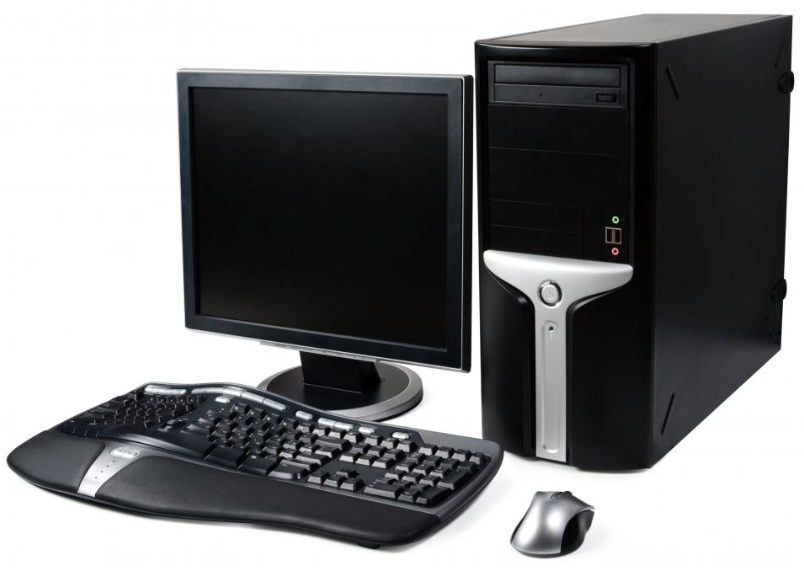
\includegraphics[height=0.8\textheight,width=0.9\textwidth,keepaspectratio]{images/desktop.png}
    \end{frame}
    
    \begin{frame}{…али то често није случај (?)}
        \centering
        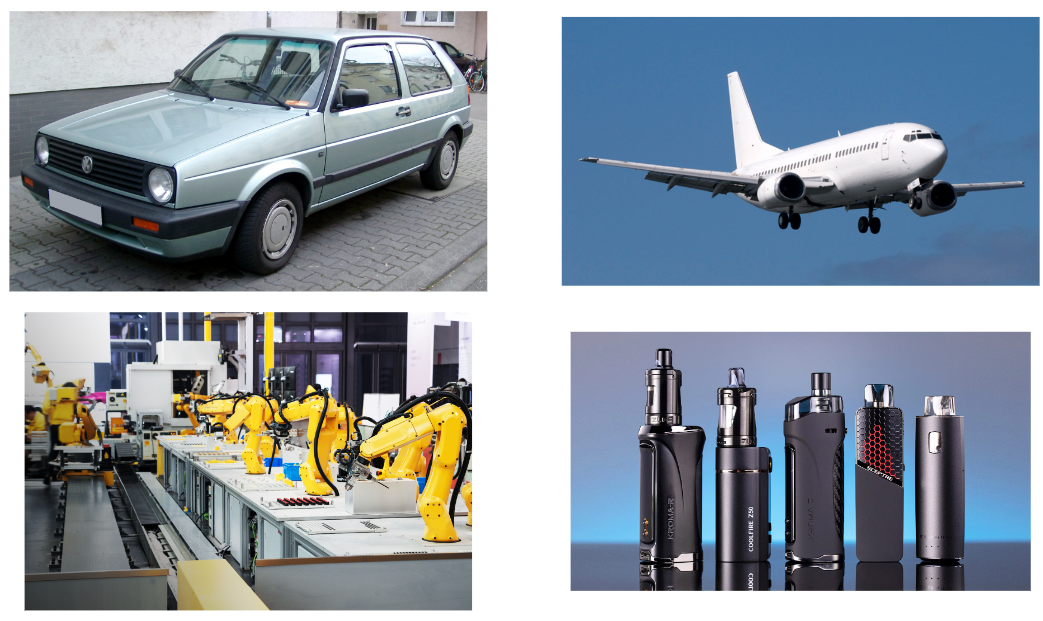
\includegraphics[height=0.8\textheight,width=0.9\textwidth,keepaspectratio]{images/embedded.png}
    \end{frame}
    
    \begin{frame}{Други покушај}
        \centering
        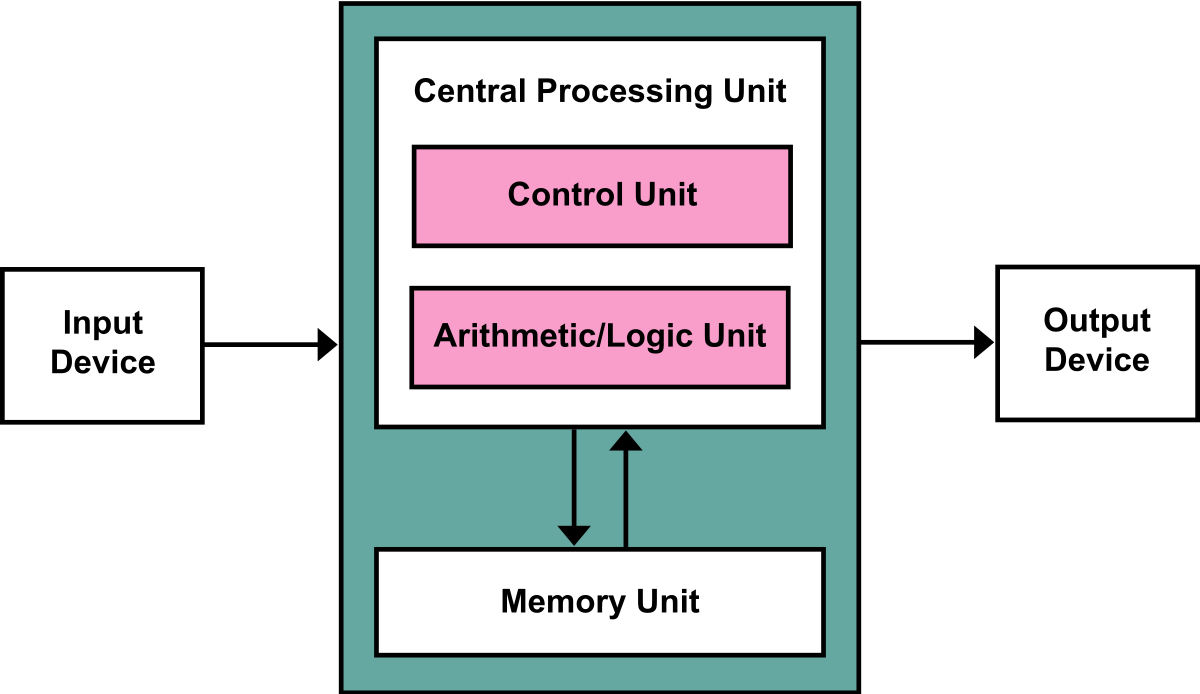
\includegraphics[height=0.8\textheight,width=0.9\textwidth,keepaspectratio]{images/von_neumann.png}
    \end{frame}
    
    \begin{frame}{Шта рачунар заиста зна да ради?}
        \begin{itemize}
            \item Језик рачунара: \textbf{скуп инструкција} (енгл. ISA, Instruction Set Architecture)
            \item Аритметичке операције: \textbf{add}, \textbf{sub}, \textbf{div}, \textbf{mul}, …
            \item Померање података:
            \begin{itemize}
                \item са улазног уређаја у меморију
                \item из меморије на излазни уређај
                \item са једне меморијске локације на другу
            \end{itemize}
            \item Условно гранање: извршавање кода уколико је логички услов испуњен
        \end{itemize}
    \end{frame}
    
    \begin{frame}{Условно гранање}
        \begin{itemize}
            \item Кључни механизам - омогућава имплементацију \textbf{било ког} алгоритма
            \item Концпети виших програмских језика као што су \textbf{if}, \textbf{else}, \textbf{for}, \textbf{while}, \textbf{switch} се своде на условно гранање
        \end{itemize}
    \end{frame}
    
    \begin{frame}{Шта је програм?}
        \textit{Рачунарски програм је \textbf{низ инструкција} садржаних у формату који рачунар може да \textbf{изврши}.}
    \end{frame}
    
    \begin{frame}{Како рачунари омогућавају аутоматизацију процеса?}
        \begin{itemize}
            \item Неопходно је да имамо формалну дефиницију процеса који желимо да аутоматизујемо - \textbf{морамо да дефинишемо алгоритам}
            \begin{itemize}
                \item сама дефиниција мора бити формална, односно мора садржати прецизан опис корака
                \item формат дефиниције не мора да буде формалан!
            \end{itemize}
            \item Формалну дефиницију морамо изразити у формату који рачунар може да изврши - \textbf{морамо да имплементирамо алгоритам}
            \item У пракси, грешке у дизајну и имплементацији су честе - \textbf{морамо да тестирамо програм}
        \end{itemize}
    \end{frame}
    
    \begin{frame}{Шта рачунар чини посебним?}
        \begin{itemize}
            \item Магија аутоматизације почива у условном гранању
            \item Ток извршавања може да се мења у зависности од вредности које нису познате за време писања програма
            \item Ове вредности називамо \textbf{променљивим}
            \item Њихове вредности морају да се налазе у меморији, како би рачунар могао да их обради, али потичу са улазних уређаја!
            \item За време писања програма, неопходно је да знамо искључиво \textbf{локацију} променљиве
        \end{itemize}
    \end{frame}
    
    \begin{frame}{Студија случаја: термостат}
        \begin{itemize}
            \item Желимо да контролишемо рад грејалице у соби у зависности од тренутне температуре
            \item Додатно, желимо да можемо да променимо жељену температуру
            \item На располагању имамо:
            \begin{itemize}
                \item \textbf{сензор температуре} - очитава тепературу у просторији
                \item \textbf{тастатуру} - омогућава унос произвољних података
                \item \textbf{микроконтролер} - једноставан рачунар на који лако можемо да повежемо сензор
                \item \textbf{релеј} - прекидач којим рачунар може да управља
            \end{itemize}
            \item Који су ваши предлози?
        \end{itemize}
    \end{frame}

\end{document}
